\documentclass[DM,lsstdraft,toc]{lsstdoc}
% lsstdoc documentation: https://lsst-texmf.lsst.io/lsstdoc.html

% Generated by Makefile
\input{meta}

% Package imports go here.
\usepackage{booktabs}
\usepackage{graphicx}

% Local commands go here.
\newcolumntype{R}[1]{>{\raggedleft\arraybackslash}p{#1}}
\newcolumntype{L}[1]{>{\raggedright\arraybackslash}p{#1}}

% If you want glossaries, uncomment:
% \input{aglossary.tex}
% \makeglossaries

\title{Characterization Metric Report: Science Pipelines Version 20.0.0}
% \setDocSubtitle{Optional subtitle}

\author{%
Jeff Carlin
}

\setDocRef{DMTR-251}
\setDocUpstreamLocation{\url{https://github.com/lsst-dm/DMTR-251}}
\date{\vcsDate}
% \setDocCurator{The Curator of this Document}

\setDocAbstract{%
This brief report describes measurements of interest that were carried out for release v20.0.0 of the Science Pipeline.
The report for the previous version can be found in \citeds{DMTR-191}.
}

% Revision history.
% Order: oldest first.
% Fields: VERSION, DATE, DESCRIPTION, OWNER NAME.
% See LPM-51 for version number policy.
\setDocChangeRecord{%
  \addtohist{1}{2020-06-16}{First Draft}{Jeff Carlin}
}

\begin{document}

\maketitle

% ADD CONTENT HERE
% You can also use the \input command to include several content files.

\section{Dashboard summary of performance metrics}

\begin{figure}
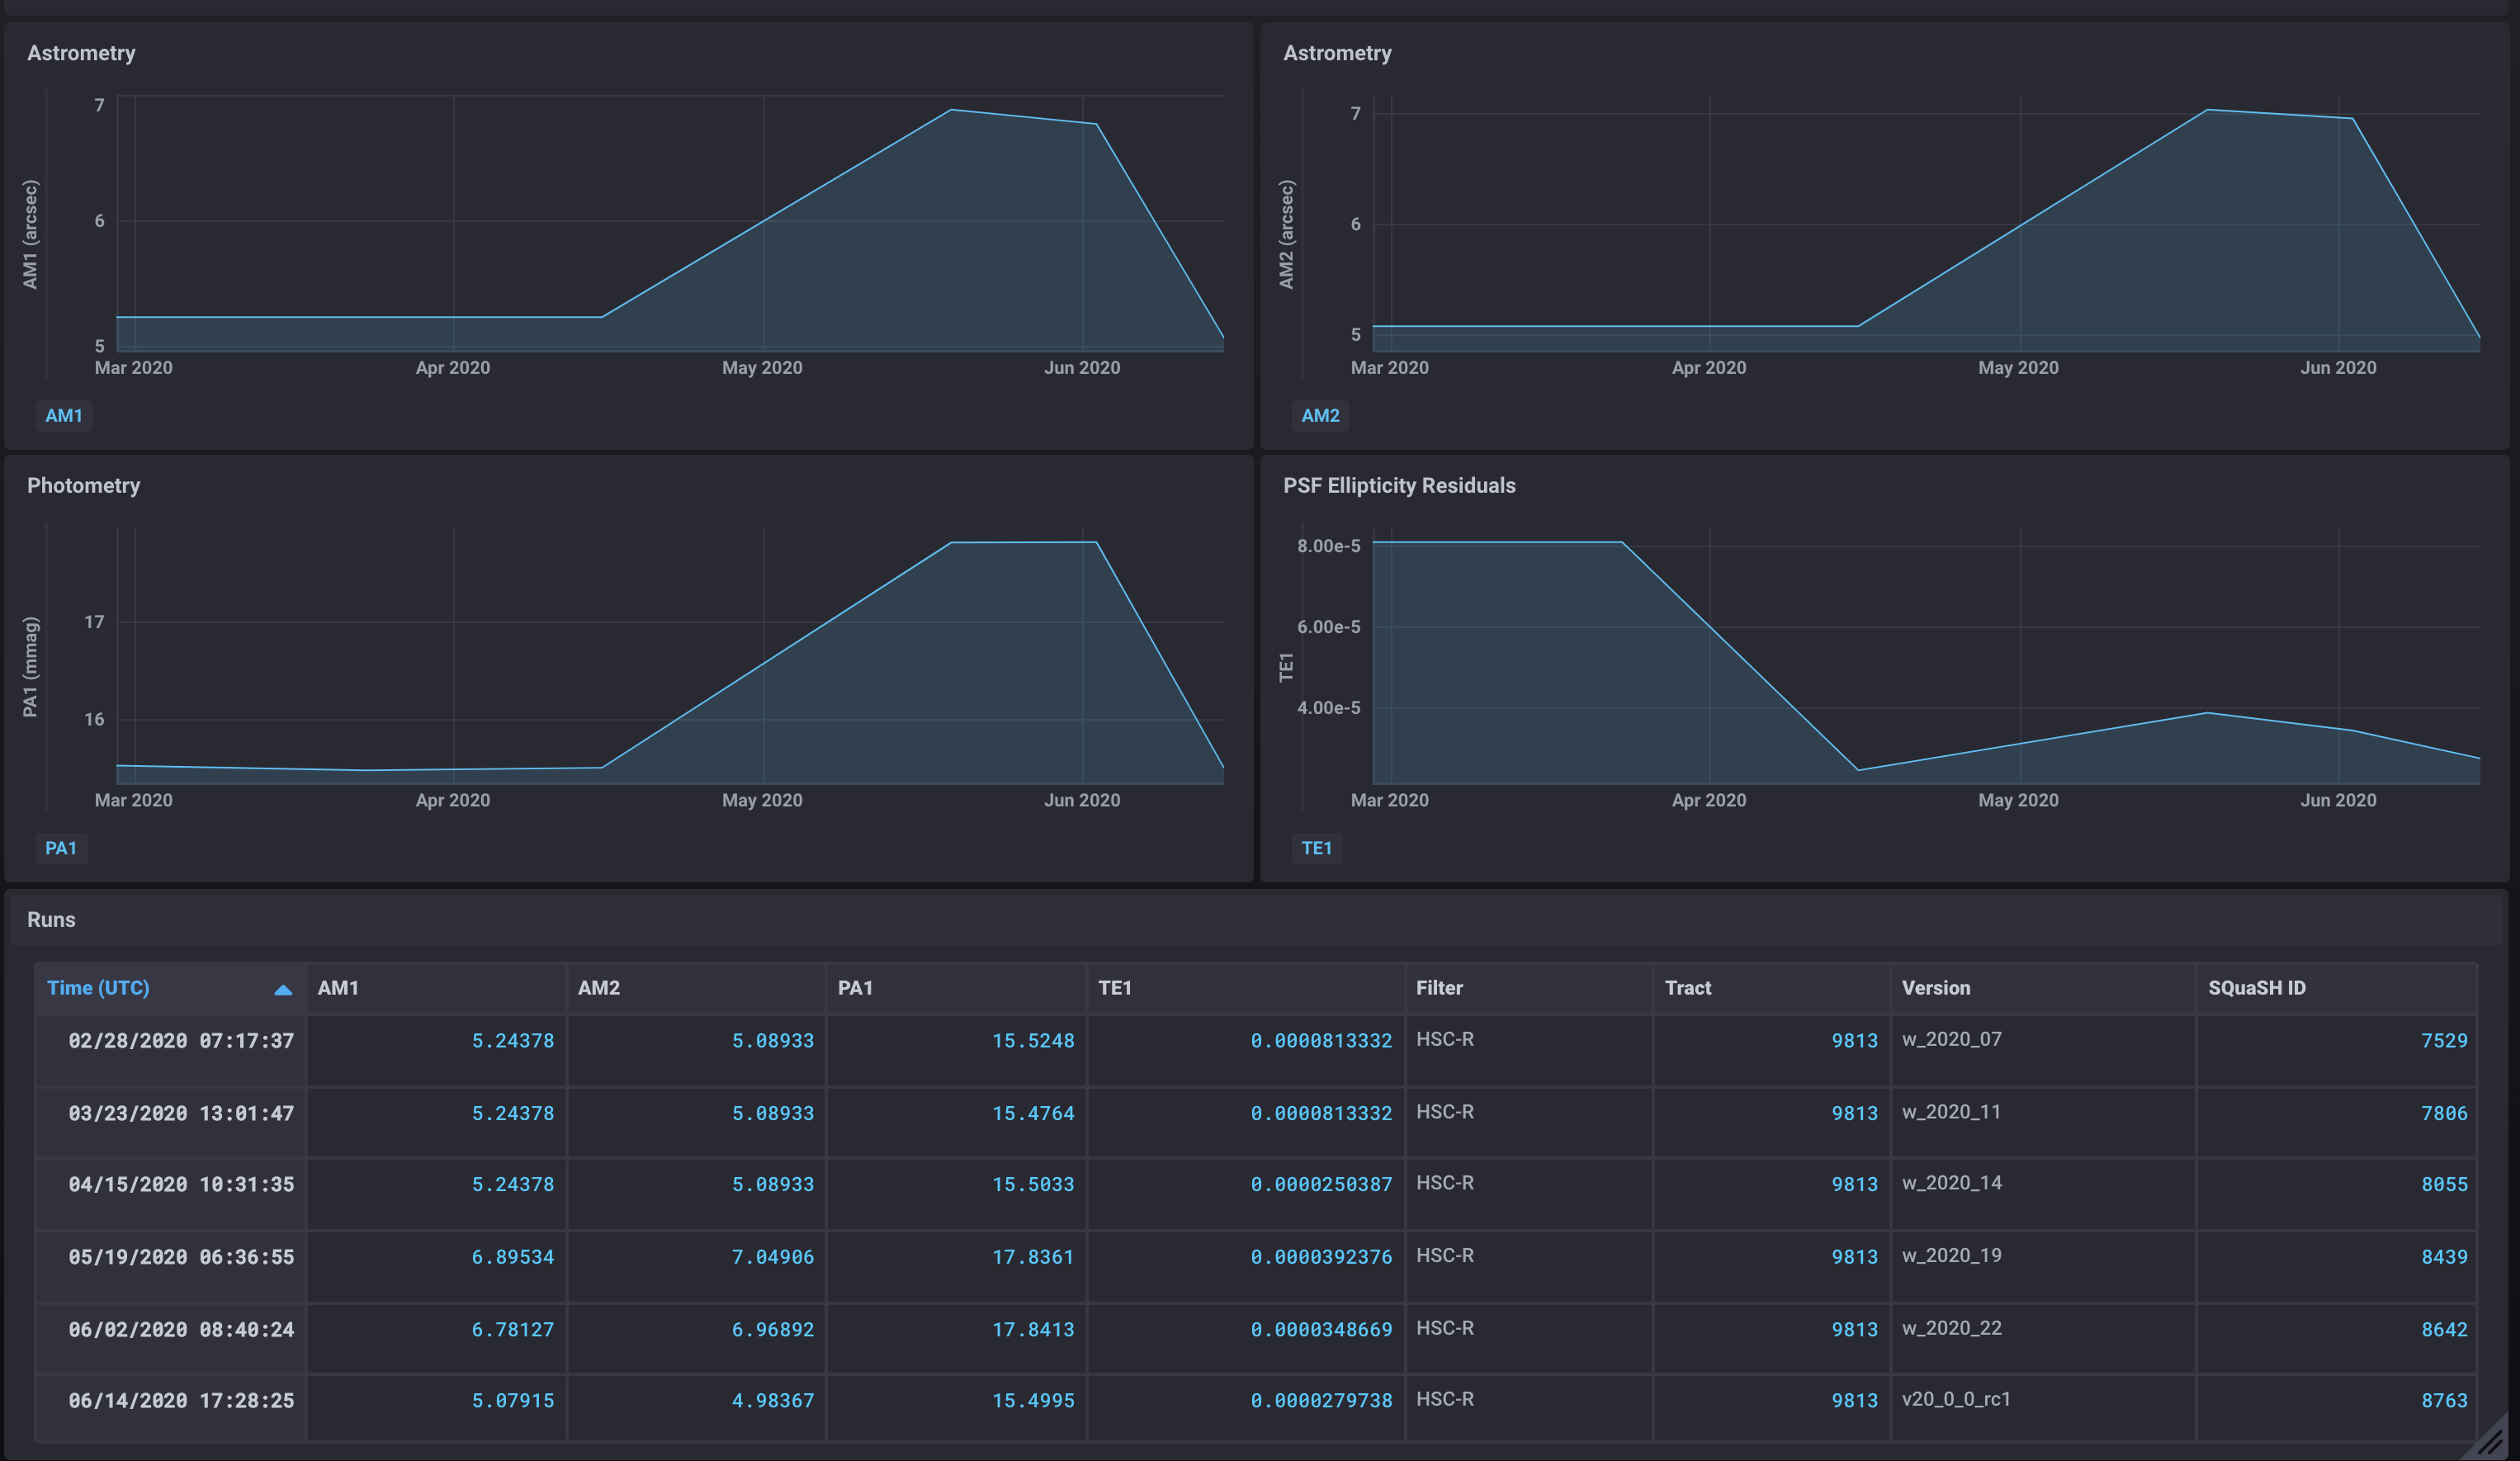
\includegraphics[width=0.9\columnwidth]{figures/SQuaSH_dashboard_RC2_tract9813.png}
\caption{}
\end{figure}

\section{Photometric Performance}\label{photometric-performance}

procCalRep corresponds to requirement OSS-REQ-0275 (defined in
\citeds{LSE-30}). All other photometric performance
metrics follow LSS-REQ-0093 (\citeds{LSE-29}) and
\citeds{LPM-17} table 14.

\begin{longtable}[]{@{}lllllll@{}}
\toprule
\begin{minipage}[b]{0.12\columnwidth}\raggedright\strut
Metric\strut
\end{minipage} & \begin{minipage}[b]{0.06\columnwidth}\raggedright\strut
Unit\strut
\end{minipage} & \begin{minipage}[b]{0.14\columnwidth}\raggedright\strut
SRD Requirement -- Design\strut
\end{minipage} & \begin{minipage}[b]{0.14\columnwidth}\raggedright\strut
Release 20 Target\strut
\end{minipage} & \begin{minipage}[b]{0.12\columnwidth}\raggedright\strut
Value (validation data)\strut
\end{minipage} & \begin{minipage}[b]{0.12\columnwidth}\raggedright\strut
Value (RC2) \strut
\end{minipage} & \begin{minipage}[b]{0.17\columnwidth}\raggedright\strut
Comments\strut
\end{minipage}\tabularnewline
\midrule
\endhead
\begin{minipage}[t]{0.12\columnwidth}\raggedright\strut
procCalRep\strut
\end{minipage} & \begin{minipage}[t]{0.06\columnwidth}\raggedright\strut
mmag\strut
\end{minipage} & \begin{minipage}[t]{0.14\columnwidth}\raggedright\strut
\(\leq 3.0\)\strut
\end{minipage} & \begin{minipage}[t]{0.14\columnwidth}\raggedright\strut
3.5\strut
\end{minipage} & \begin{minipage}[t]{0.12\columnwidth}\raggedright\strut
---\strut
\end{minipage} & \begin{minipage}[t]{0.12\columnwidth}\raggedright\strut
---\strut
\end{minipage} & \begin{minipage}[t]{0.17\columnwidth}\raggedright\strut
Need simulations\strut
\end{minipage}\tabularnewline
\begin{minipage}[t]{0.12\columnwidth}\raggedright\strut
PA1: \emph{u}\strut
\end{minipage} & \begin{minipage}[t]{0.06\columnwidth}\raggedright\strut
mmag\strut
\end{minipage} & \begin{minipage}[t]{0.14\columnwidth}\raggedright\strut
\(\leq 7.5\)\strut
\end{minipage} & \begin{minipage}[t]{0.14\columnwidth}\raggedright\strut
8.0\strut
\end{minipage} & \begin{minipage}[t]{0.12\columnwidth}\raggedright\strut
---\strut
\end{minipage} & \begin{minipage}[t]{0.12\columnwidth}\raggedright\strut
1.0 \strut
\end{minipage} & \begin{minipage}[t]{0.17\columnwidth}\raggedright\strut
No data\strut
\end{minipage}\tabularnewline
\begin{minipage}[t]{0.12\columnwidth}\raggedright\strut
PA1: \emph{g}\strut
\end{minipage} & \begin{minipage}[t]{0.06\columnwidth}\raggedright\strut
mmag\strut
\end{minipage} & \begin{minipage}[t]{0.14\columnwidth}\raggedright\strut
\(\leq 5.0\)\strut
\end{minipage} & \begin{minipage}[t]{0.14\columnwidth}\raggedright\strut
5.5\strut
\end{minipage} & \begin{minipage}[t]{0.12\columnwidth}\raggedright\strut
---\strut
\end{minipage} & \begin{minipage}[t]{0.12\columnwidth}\raggedright\strut
12.7 \strut
\end{minipage} & \begin{minipage}[t]{0.17\columnwidth}\raggedright\strut
\strut
\end{minipage}\tabularnewline
\begin{minipage}[t]{0.12\columnwidth}\raggedright\strut
PA1: \emph{r}\strut
\end{minipage} & \begin{minipage}[t]{0.06\columnwidth}\raggedright\strut
mmag\strut
\end{minipage} & \begin{minipage}[t]{0.14\columnwidth}\raggedright\strut
\(\leq 5.0\)\strut
\end{minipage} & \begin{minipage}[t]{0.14\columnwidth}\raggedright\strut
5.5\strut
\end{minipage} & \begin{minipage}[t]{0.12\columnwidth}\raggedright\strut
13.7\strut
\end{minipage} & \begin{minipage}[t]{0.12\columnwidth}\raggedright\strut
14.1\strut
\end{minipage} & \begin{minipage}[t]{0.17\columnwidth}\raggedright\strut
\strut
\end{minipage}\tabularnewline
\begin{minipage}[t]{0.12\columnwidth}\raggedright\strut
PA1: \emph{i}\strut
\end{minipage} & \begin{minipage}[t]{0.06\columnwidth}\raggedright\strut
mmag\strut
\end{minipage} & \begin{minipage}[t]{0.14\columnwidth}\raggedright\strut
\(\leq 5.0\)\strut
\end{minipage} & \begin{minipage}[t]{0.14\columnwidth}\raggedright\strut
5.5\strut
\end{minipage} & \begin{minipage}[t]{0.12\columnwidth}\raggedright\strut
12.1\strut
\end{minipage} & \begin{minipage}[t]{0.12\columnwidth}\raggedright\strut
14.0\strut
\end{minipage} & \begin{minipage}[t]{0.17\columnwidth}\raggedright\strut
\strut
\end{minipage}\tabularnewline
\begin{minipage}[t]{0.12\columnwidth}\raggedright\strut
PA1: \emph{z}\strut
\end{minipage} & \begin{minipage}[t]{0.06\columnwidth}\raggedright\strut
mmag\strut
\end{minipage} & \begin{minipage}[t]{0.14\columnwidth}\raggedright\strut
\(\leq 7.5\)\strut
\end{minipage} & \begin{minipage}[t]{0.14\columnwidth}\raggedright\strut
8.0\strut
\end{minipage} & \begin{minipage}[t]{0.12\columnwidth}\raggedright\strut
---\strut
\end{minipage} & \begin{minipage}[t]{0.12\columnwidth}\raggedright\strut
11.6\strut
\end{minipage} & \begin{minipage}[t]{0.17\columnwidth}\raggedright\strut
\strut
\end{minipage}\tabularnewline
\begin{minipage}[t]{0.12\columnwidth}\raggedright\strut
PA1: \emph{y}\strut
\end{minipage} & \begin{minipage}[t]{0.06\columnwidth}\raggedright\strut
mmag\strut
\end{minipage} & \begin{minipage}[t]{0.14\columnwidth}\raggedright\strut
\(\leq 7.5\)\strut
\end{minipage} & \begin{minipage}[t]{0.14\columnwidth}\raggedright\strut
8.0\strut
\end{minipage} & \begin{minipage}[t]{0.12\columnwidth}\raggedright\strut
23.8\strut
\end{minipage} & \begin{minipage}[t]{0.12\columnwidth}\raggedright\strut
13.5\strut
\end{minipage} & \begin{minipage}[t]{0.17\columnwidth}\raggedright\strut
\strut
\end{minipage}\tabularnewline
\begin{minipage}[t]{0.12\columnwidth}\raggedright\strut
PF1: \emph{u}\strut
\end{minipage} & \begin{minipage}[t]{0.06\columnwidth}\raggedright\strut
\%\strut
\end{minipage} & \begin{minipage}[t]{0.14\columnwidth}\raggedright\strut
\(\leq 20\)\strut
\end{minipage} & \begin{minipage}[t]{0.14\columnwidth}\raggedright\strut
---\strut
\end{minipage} & \begin{minipage}[t]{0.12\columnwidth}\raggedright\strut
---\strut
\end{minipage} & \begin{minipage}[t]{0.12\columnwidth}\raggedright\strut
---\strut
\end{minipage} & \begin{minipage}[t]{0.17\columnwidth}\raggedright\strut
No data\strut
\end{minipage}\tabularnewline
\begin{minipage}[t]{0.12\columnwidth}\raggedright\strut
PF1: \emph{g}\strut
\end{minipage} & \begin{minipage}[t]{0.06\columnwidth}\raggedright\strut
\%\strut
\end{minipage} & \begin{minipage}[t]{0.14\columnwidth}\raggedright\strut
\(\leq 20\)\strut
\end{minipage} & \begin{minipage}[t]{0.14\columnwidth}\raggedright\strut
---\strut
\end{minipage} & \begin{minipage}[t]{0.12\columnwidth}\raggedright\strut
---\strut
\end{minipage} & \begin{minipage}[t]{0.12\columnwidth}\raggedright\strut
28.6\strut
\end{minipage} & \begin{minipage}[t]{0.17\columnwidth}\raggedright\strut
\strut
\end{minipage}\tabularnewline
\begin{minipage}[t]{0.12\columnwidth}\raggedright\strut
PF1: \emph{r}\strut
\end{minipage} & \begin{minipage}[t]{0.06\columnwidth}\raggedright\strut
\%\strut
\end{minipage} & \begin{minipage}[t]{0.14\columnwidth}\raggedright\strut
\(\leq 10\)\strut
\end{minipage} & \begin{minipage}[t]{0.14\columnwidth}\raggedright\strut
10.0\strut
\end{minipage} & \begin{minipage}[t]{0.12\columnwidth}\raggedright\strut
30.1\strut
\end{minipage} & \begin{minipage}[t]{0.12\columnwidth}\raggedright\strut
31.1\strut
\end{minipage} & \begin{minipage}[t]{0.17\columnwidth}\raggedright\strut
\strut
\end{minipage}\tabularnewline
\begin{minipage}[t]{0.12\columnwidth}\raggedright\strut
PF1: \emph{i}\strut
\end{minipage} & \begin{minipage}[t]{0.06\columnwidth}\raggedright\strut
\%\strut
\end{minipage} & \begin{minipage}[t]{0.14\columnwidth}\raggedright\strut
\(\leq 10\)\strut
\end{minipage} & \begin{minipage}[t]{0.14\columnwidth}\raggedright\strut
10.0\strut
\end{minipage} & \begin{minipage}[t]{0.12\columnwidth}\raggedright\strut
25.9\strut
\end{minipage} & \begin{minipage}[t]{0.12\columnwidth}\raggedright\strut
31.7\strut
\end{minipage} & \begin{minipage}[t]{0.17\columnwidth}\raggedright\strut
\strut
\end{minipage}\tabularnewline
\begin{minipage}[t]{0.12\columnwidth}\raggedright\strut
PF1: \emph{z}\strut
\end{minipage} & \begin{minipage}[t]{0.06\columnwidth}\raggedright\strut
\%\strut
\end{minipage} & \begin{minipage}[t]{0.14\columnwidth}\raggedright\strut
\(\leq 20\)\strut
\end{minipage} & \begin{minipage}[t]{0.14\columnwidth}\raggedright\strut
---\strut
\end{minipage} & \begin{minipage}[t]{0.12\columnwidth}\raggedright\strut
---\strut
\end{minipage} & \begin{minipage}[t]{0.12\columnwidth}\raggedright\strut
13.2\strut
\end{minipage} & \begin{minipage}[t]{0.17\columnwidth}\raggedright\strut
\strut
\end{minipage}\tabularnewline
\begin{minipage}[t]{0.12\columnwidth}\raggedright\strut
PF1: \emph{y}\strut
\end{minipage} & \begin{minipage}[t]{0.06\columnwidth}\raggedright\strut
\%\strut
\end{minipage} & \begin{minipage}[t]{0.14\columnwidth}\raggedright\strut
\(\leq 10\)\strut
\end{minipage} & \begin{minipage}[t]{0.14\columnwidth}\raggedright\strut
10.0\strut
\end{minipage} & \begin{minipage}[t]{0.12\columnwidth}\raggedright\strut
34.7\strut
\end{minipage} & \begin{minipage}[t]{0.12\columnwidth}\raggedright\strut
16.6\strut
\end{minipage} & \begin{minipage}[t]{0.17\columnwidth}\raggedright\strut
\strut
\end{minipage}\tabularnewline
\begin{minipage}[t]{0.12\columnwidth}\raggedright\strut
PA2: \emph{u}\strut
\end{minipage} & \begin{minipage}[t]{0.06\columnwidth}\raggedright\strut
\%\strut
\end{minipage} & \begin{minipage}[t]{0.14\columnwidth}\raggedright\strut
\(\leq 22.5\)\strut
\end{minipage} & \begin{minipage}[t]{0.14\columnwidth}\raggedright\strut
---\strut
\end{minipage} & \begin{minipage}[t]{0.12\columnwidth}\raggedright\strut
---\strut
\end{minipage} & \begin{minipage}[t]{0.12\columnwidth}\raggedright\strut
---\strut
\end{minipage} & \begin{minipage}[t]{0.17\columnwidth}\raggedright\strut
No data\strut
\end{minipage}\tabularnewline
\begin{minipage}[t]{0.12\columnwidth}\raggedright\strut
PA2: \emph{g}\strut
\end{minipage} & \begin{minipage}[t]{0.06\columnwidth}\raggedright\strut
\%\strut
\end{minipage} & \begin{minipage}[t]{0.14\columnwidth}\raggedright\strut
\(\leq 15\)\strut
\end{minipage} & \begin{minipage}[t]{0.14\columnwidth}\raggedright\strut
---\strut
\end{minipage} & \begin{minipage}[t]{0.12\columnwidth}\raggedright\strut
---\strut
\end{minipage} & \begin{minipage}[t]{0.12\columnwidth}\raggedright\strut
27.9\strut
\end{minipage} & \begin{minipage}[t]{0.17\columnwidth}\raggedright\strut
\strut
\end{minipage}\tabularnewline
\begin{minipage}[t]{0.12\columnwidth}\raggedright\strut
PA2: \emph{r}\strut
\end{minipage} & \begin{minipage}[t]{0.06\columnwidth}\raggedright\strut
\%\strut
\end{minipage} & \begin{minipage}[t]{0.14\columnwidth}\raggedright\strut
\(\leq 15\)\strut
\end{minipage} & \begin{minipage}[t]{0.14\columnwidth}\raggedright\strut
20.0\strut
\end{minipage} & \begin{minipage}[t]{0.12\columnwidth}\raggedright\strut
26.6\strut
\end{minipage} & \begin{minipage}[t]{0.12\columnwidth}\raggedright\strut
29.8\strut
\end{minipage} & \begin{minipage}[t]{0.17\columnwidth}\raggedright\strut
\strut
\end{minipage}\tabularnewline
\begin{minipage}[t]{0.12\columnwidth}\raggedright\strut
PA2: \emph{i}\strut
\end{minipage} & \begin{minipage}[t]{0.06\columnwidth}\raggedright\strut
\%\strut
\end{minipage} & \begin{minipage}[t]{0.14\columnwidth}\raggedright\strut
\(\leq 15\)\strut
\end{minipage} & \begin{minipage}[t]{0.14\columnwidth}\raggedright\strut
20.0\strut
\end{minipage} & \begin{minipage}[t]{0.12\columnwidth}\raggedright\strut
25.4\strut
\end{minipage} & \begin{minipage}[t]{0.12\columnwidth}\raggedright\strut
29.7\strut
\end{minipage} & \begin{minipage}[t]{0.17\columnwidth}\raggedright\strut
\strut
\end{minipage}\tabularnewline
\begin{minipage}[t]{0.12\columnwidth}\raggedright\strut
PA2: \emph{z}\strut
\end{minipage} & \begin{minipage}[t]{0.06\columnwidth}\raggedright\strut
\%\strut
\end{minipage} & \begin{minipage}[t]{0.14\columnwidth}\raggedright\strut
\(\leq 22.5\)\strut
\end{minipage} & \begin{minipage}[t]{0.14\columnwidth}\raggedright\strut
---\strut
\end{minipage} & \begin{minipage}[t]{0.12\columnwidth}\raggedright\strut
---\strut
\end{minipage} & \begin{minipage}[t]{0.12\columnwidth}\raggedright\strut
25.5\strut
\end{minipage} & \begin{minipage}[t]{0.17\columnwidth}\raggedright\strut
\strut
\end{minipage}\tabularnewline
\begin{minipage}[t]{0.12\columnwidth}\raggedright\strut
PA2: \emph{y}\strut
\end{minipage} & \begin{minipage}[t]{0.06\columnwidth}\raggedright\strut
\%\strut
\end{minipage} & \begin{minipage}[t]{0.14\columnwidth}\raggedright\strut
\(\leq 22.5\)\strut
\end{minipage} & \begin{minipage}[t]{0.14\columnwidth}\raggedright\strut
22.5\strut
\end{minipage} & \begin{minipage}[t]{0.12\columnwidth}\raggedright\strut
41.3\strut
\end{minipage} & \begin{minipage}[t]{0.12\columnwidth}\raggedright\strut
29.6\strut
\end{minipage} & \begin{minipage}[t]{0.17\columnwidth}\raggedright\strut
\strut
\end{minipage}\tabularnewline

\end{longtable}


\appendix

% Include all the relevant bib files.
% https://lsst-texmf.lsst.io/lsstdoc.html#bibliographies
\section{References} \label{sec:bib}
\renewcommand{\refname}{} % Suppress default Bibliography section
\bibliography{local,lsst,lsst-dm,refs_ads,refs,books}

% Make sure lsst-texmf/bin/generateAcronyms.py is in your path
\section{Acronyms} \label{sec:acronyms}
\input{acronyms.tex}
% If you want glossary uncomment below and comment out the two lines above.
% \printglossaries

\end{document}
